\section{Introduction}~\label{sec:intro}

% the problems of patch management 
% why do we need to patch 
% vulnerabilities faster -- EQUIFAX
Delays in deploying patches to known software security vulnerabilities 
have been the cause of major cybersecurity attacks~\cite{windows-cyberattack,failed-to-deploy-patch,hacker-news-patches,CISA-ALERT,non-applied-patches}. 
A practical example with major financial and reputation losses was the Equifax breach~\cite{failed-to-deploy-patch}: a failure to patch a 2-month-old critical bug in Apache Struts, which led to a sensitive data breach that impacted more than 143 million US consumers~\cite{EQUIFAX-1}. 
Timely patch management (i.e., the fast distribution and deployment 
of security fixes to users~\cite{SOFT-PATCH-MANAG-NIST,DBLP:conf/soups/LiRMMC19,10.5555/3488905.3488919,10.5555/3337432.3337437}) is one of the most effective and widely recognized strategies for 
% reducing the users' exposure window~\cite{DBLP:journals/corr/abs-2001-09148} and 
protecting
software systems against  cyberattacks~\cite{DISSANAYAKE2022106771,SOFT-PATCH-MANAG-NIST}. Yet, one important challenge still prevails, the \emph{lack of efficient patch triage systems} to identify and prioritize security patches~\cite{Zhang2021AnIO, SSPatcher2022,hacker-news-patches,DBLP:conf/soups/LiRMMC19}: current processes are largely manual (time-consuming) and prone to ignore important bug fixes such as the one behind Equifax~\cite{failed-to-deploy-patch}. An ideal and effective patch management process should include an effective audit system to identify patches~\cite{hacker-news-patches}. A recent study showed that $56.7\%$ of the commit messages attached to security patches are documented poorly and hinder  triage systems tasks (e.g., detection, prioritization, and assessment)~\cite{10.1145/3593434.3593481}.  

\textbf{Problem: Poor quality security commit messages hinder patch triage systems.} Previous work focused on using 
patch metadata (e.g., commit message) and code changes 
to explore automated patch detection~\cite{SSPatcher2022,reis2017secbench,9678720,DBLP:journals/corr/abs-1806-05893}, concluded that software vulnerability management (SVM) techniques could not rely purely on metadata to detect software vulnerabilities
due to the often inaccurate and incomplete  data~\cite{DBLP:journals/corr/abs-1806-05893}. In fact, only $38\%$ of commit messages used to ``silently'' patch software vulnerabilities in the past included security-related words~\cite{9678720}. Silent fixes
are performed when the vendor patches a vulnerability  without mentioning its existence anywhere (e.g., release notes, commit message, and more)~\cite{9678720}. This practice naturally leads to less informative patch documentation and hinders triage systems awareness and effectiveness. While this practice is usually used to protect vendors and systems, it
also limits the general knowledge pool of people who actually understand the vulnerability and know how to exploit it, which leaves users and defenders unprotected and unaware. According to the CERT Coordinated Vulnerability Disclosure (CVD) guide, silent patches should be avoided since knowing the existence of vulnerabilities and their patches is often the key driver to effective patch deployment~\cite{Householder2020}. 

%%%% Importance of the problem
% Providing well-structured and quality documentation of security patches can improve the  understanding of these software vulnerabilities for researchers and developers, which can ultimately enable faster patch management~\cite{Zhang2021AnIO,Householder2020,SSPatcher2022,10.1145/3593434.3593481}. Software vulnerabilities are, on average, disclosed only one week after the patch release~\cite{10.1145/3133956.3134072}---leaving, again, users vulnerable and unaware. Therefore, making the information available earlier in the process is of utmost importance.

%%%% not sure how this part helps
% Yet, previous work succeeded in locating software vulnerabilities and their respective patches using manual validation~\cite{10.1109/MSR.2019.00064} or regular expressions~\cite{reis2017secbench, SSPatcher2022} over commit messages (i.e., some data in commit messages can in fact be leveraged for this task).

\textbf{Motivation:} 
Security commit messages (i.e., the commit messages attached to the code changes used to patch software vulnerabilities) can be cryptic~\cite{9678720}, hindering triage tasks. 
Table~\ref{tab:messages} shows examples of security commit messages (col. Message) used to document patches to known software vulnerabilities (col. VulnID) and the 
patch commit key (col. SHA). Message 1 (``.'') is an example of a cryptic message as it does not provide any information. From messages 2 and 3, it
is possible to infer that a defect in code is being fixed, but nothing 
more than that. Message 4 is an internet meme called ``Rickrolling''\footnote{``Rickrolling'' meme details at \url{https://knowyourmeme.com/memes/rickroll}}, usually used to prank people with the "Never Gonna Give You Up" song. Although funny, the message does not provide, again, any relevant information regarding the vulnerability and respective patch. Most of the cases presented would not be detected by triage systems leaving users unaware of the new patches and exposed to vulnerabilities. Message 5  
provides a brief description of the patch and some relevant information about it (e.g., it fixes a ``security issue'' related to ``passwords''). The respective code changes fix a potential buffer overrun vulnerability resulting from reading user-provided passwords and confirmations via command-line prompts. The patch fixes an ``Improper Authentication'' weakness (CWE-287) with a severity (CVSS) score of $8.4$ in $10$---which 
is not explicit in the message. This extra information could have helped
automated or even manual patch triage systems to prioritize this patch since it has high severity. 



\begin{table}[!t]
    \footnotesize
    \centering
    \begin{tabular}{ | p{0.01cm} | p{4.8cm} | p{1.5cm} | p{0.9cm} |} 
    \hline
     & \textbf{Commit Message} & \textbf{VulnID} & \textbf{SHA}\\\hline
        1 & \texttt{.} & CVE-2019-13568 & \href{https://github.com/GreycLab/CImg/commit/ac8003393569aba51048c9d67e1491559877b1d1}{ac80033} \\\hline
        2 & \texttt{Minor patch.} & OSV-2020-2108 & \href{https://github.com/simdjson/simdjson/commit/a8bf10ea5a0ea2553f07ac46744666c94d0085fc}{a8bf10e} \\\hline
        3 & \texttt{Code refactoring.} & GHSA-4fc4-4p5g-6w89 & \href{https://github.com/ckeditor/ckeditor4/commit/d158413449692d920a778503502dcb22881bc949}{d158413} \\\hline
        4 & \texttt{<scratchsig><script>location=
        'https:\/\/www.youtube.com\/watch?
        v=dQw4w9WgXcQ';<\/script><\/scratchsig>} & CVE-2020-15179 & \href{https://github.com//InternationalScratchWiki//wiki-scratchsig//commit//4160a39a20eebeb63a59eb7597a91b961eca6388}{4160a39} \\\hline
        5 & \texttt{Fixed security issues with passwords entered via a prompt} & CVE-2022-35928 & \href{https://github.com/paulej/AESCrypt/commit/68761851b595e96c68c3f46bfc21167e72c6a22c}{6876185} \\
    \hline
    \end{tabular}
    \caption{Examples of commit messages used to patch known software vulnerabilities.}
    \label{tab:messages}
\end{table}


\textbf{Study.} While some argue that security commit messages and patch release notes should be minimalist, others argue that the details are crucial to ensure triage systems effectiveness~\cite{SSPatcher2022,Zhang2021AnIO}, create trust amongst users~\cite{Householder2020}, and enable fast patch management~\cite{Zhang2021AnIO,Householder2020}. Therefore, we investigated the current status of security commit messages and answered the following questions: (1) what information is included in commit messages of public security patches; (2) are security engineers following best practices to produce security commit messages; and, 
(3) is the security community open to a new
standard for security commit messages.
In our work, we empirically analyzed $11036$ security commit messages by extracting key information (security words, vulnerability ID, weakness ID, severity, and more) with a customized named entity recognition (NER) tool.

\textbf{Results.} We found that $61.2\%$ of security commit messages include security-related words but lack key information such as the vulnerability ID, weakness ID, and severity. We were unable to extract any information from $8\%$ of the messages because (1) they were poorly documented, (2) their vocabulary was non-security related, or (3) they had misspelled words. Overall, security engineers poorly follow best practices to write general commit messages indicating that a set of new best practices for this task are needed. 

\textbf{Solution.} To address the challenges identified from our empirical analysis, we developed a structured and comprehensive convention called \texttt{SECOM} for writing security commit messages. We noticed 
security engineers sometimes follow standards to write general commit messages in security commit messages (e.g., Conventional Commits~\cite{convcom}). Therefore, we designed the standard
on top of best practices for writing generic commit messages to facilitate adoption. \texttt{SECOM} was designed according to (1) the results of the empirical analysis of historical commit messages and (2) validation of SECOM with the open-source security community. The standard was created with the aim of making the task of automated reasoning tools easier for patch detection (by adding a clear indicator for vulnerability fixes) and prioritization (by considering severity score and weakness type). 

\begin{figure}[!t]
    \centering
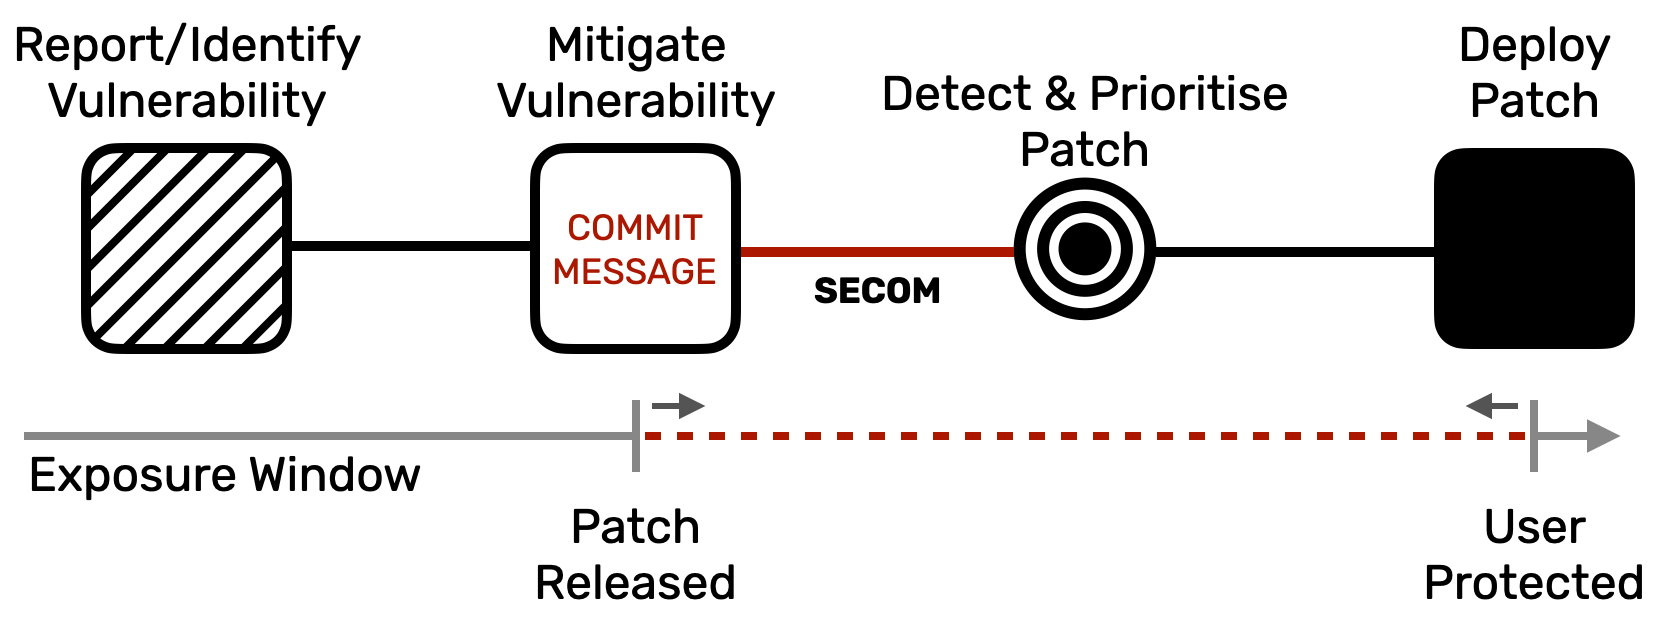
\includegraphics[width=\linewidth]{Figures/cycle.png}
    \caption{Problem and Solution illustration.}\label{fig:cycle}
\end{figure}

\textbf{Impact.} Figure~\ref{fig:cycle} shows where SECOM can help improve patch management processes: well-documented commit messages can be detected by triage systems and shorten the time between the patch is released and deployed. 
From a research perspective, detecting and assessing vulnerabilities continues to be a main challenge in vulnerability prediction due to the scarcity
and poor quality of curated data~\cite{9448435}. 
\texttt{SECOM} can be an important tool in softening this issue since it has the potential to improve the quality of data for future dataset creation. More than 2k security commit messages have been produced with the \texttt{SECOM} convention\footnote{\url{https://github.com/JLLeitschuh/security-research/issues/8}} so far.
We are aware of the challenges that come from too much transparency, and we want to guide the community to make proper and careful use of this new standard. Therefore, in this paper, we also provide guidelines on using \texttt{SECOM} carefully.
% Efforts to automate compliance validation and recommendations are also mentioned in this paper. 

\textbf{Contribution.} In summary, our contributions are the following: 
(1) an empirical analysis of security commit messages and best practices application; (2) a standard for security commit messages, called SECOM; and, (3) guidelines on how to write better security commit messages and apply the convention carefully.



\section{Background}~\label{sec:background}

This section provides background information on the Named Entity Recognition (NER) theory, the approach used to extract key information from security commit messages.

\subsection{Named Entity Recognition}~\label{sec:ner}

\begin{figure}[t!]
\hspace*{-0.25cm}\centering
    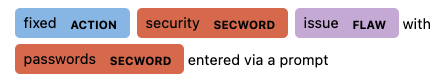
\includegraphics[width=\linewidth]{Figures/application.png}
    \caption{Named Entity Recognition (NER) application example for a security commit message.}\label{fig:application}
\end{figure}

Named Entity Recognition (NER) is a form of
Natural Language Processing (NLP)---also referred to as entity chunking, extraction, or identification. It is the task of identifying and extracting key information, called \emph{entities}, from unstructured data (in this case, text)~\cite{9039685, mikheev-etal-1999-named, lample-etal-2016-neural}.

An \emph{entity} can be any word or bag of words that refer to the same \emph{entity category}. For instance, different names of companies ``Netflix'', ``Google'' or ``Apple'' are entities that belong to the \emph{Company} category. 
NER requires the design of specific entity categories and the respective entity values, which relies on good domain knowledge. 
NER has been applied to different domains in the past, such as biomedical sciences~\cite{hakala-pyysalo-2019-biomedical}, pharmacology~\cite{gonzalez-agirre-etal-2019-pharmaconer}, and even security. 

\subsection{Named Entity Recognition in Security}~\label{sec:ner}

Previous work used NER to extract product names and versions from vulnerability reports~\cite{10.5555/3361338.3361399}. In our empirical analysis, we designed a group of category entities that are usually found in security commit messages and used a customized NER tool for security to extract key information (or entities) from commit messages used to patch software vulnerabilities.
Figure~\ref{fig:application}
shows an example of how we applied NER to security commit messages. Our tool extracted 4 different entities (``fixed'', ``security'', ``issue'', ``passwords'') for 3 different category entities (``ACTION'', ``SECWORD'', ``FLAW''). Only relevant words are extracted and tagged with their respective category entities, which is crucial for a  better understanding of the meaningful information provided in security commit messages.


\section{Research Questions}\label{sec:research_questions}

We use a mixed-method approach to answer three research questions. The first two research questions, RQ1 and RQ2, are answered by a cross-sectional empirical study of existing security commit messages. The third research question, RQ3, is answered through a survey study. 

\subsubsection*{\textbf{RQ1. What information is included in
the commit messages of public security patches?}}

Previous work has shown that SVM techniques can not rely purely on commit messages due to poor data quality~\cite{DBLP:journals/corr/abs-1806-05893}.
A study on vulnerabilities patched ``silently'' showed that only $38\%$ of commit messages used to fix vulnerabilities included security-related words~\cite{9678720}. 
But some previous approaches have managed to find some relevant natural language information in commit messages and perform security patch detection~\cite{reis2017secbench,10.1145/3106237.3117771,SSPatcher2022,DBLP:journals/corr/abs-1807-02458,10.1145/3593434.3593481}. The question 
that remains is what information is being mentioned in the commit messages
of security patches.

% \textbf{RQ2. Are there any guidelines available to
% produce security commit messages?} One way to produce quality 
% commit messages is by following best practices or guidelines~\cite{Tian_2022, convcom,linus,atomic}. In this part
% of the study, we searched for potential 
% standards to write commit messages of software security patches.

\textbf{RQ2. Do security engineers follow best practices to write security commit
messages?} 
One way to produce quality 
commit messages is by following best practices or guidelines~\cite{Tian_2022, convcom,linus,atomic}. However, researchers found that $44\%$ of commit messages need improvement~\cite{Tian_2022}. 
Our research revealed a lack of standards for writing security commit messages. Instead,
we found standards and guidelines for generic commit messages~\cite{convcom, linus, goodcommit}.
%In this part of our empirical analysis, 
Therefore, we explored if available guidelines or standards 
were being used and how they could be leveraged to create more structured and complete commit messages for security patches.

\emph{\textbf{RQ3. How open is the security community to a new standard for security commit messages?}}. Standards are usually seen as a burden or with resistance. However, in order to fix challenges, we need to create them. Therefore, we validated our convention with the open-source security community (Open Source
Security Foundation).


\section{Study of Existing Security Commit Messages}\label{sec:study_design}

This section describes an exploratory, cross-sectional empirical study of security commit messages collected from security patches for known vulnerabilities for answering RQ1 and RQ2. 


\subsection{Dataset Collection and Preprocessing} 

This section presents the steps taken to create a dataset of security commit messages.
All the tools used to collect and preprocess the data are available in our replication package. Our dataset considers data released until the 12th of August, 2022.
We collected security commit messages for our exploratory analysis by following the steps described below.

\subsubsection{Vulnerability Metadata Collection from Public Vulnerability Databases}
%
Public vulnerability databases, such as 
the National Vulnerability Database 
(NVD)~\cite{nvd}, and
the Open-Source Vulnerability (OSV) 
database~\cite{osv}, integrate documentation (or reports) for thousands of known vulnerabilities. Our dump of the OSV database includes a total of $30091$ vulnerability reports for open-source vulnerabilities from different ecosystems:
$28.6\%$ of the vulnerabilities were reported by GitHub Advisories, $25.7\%$ by  Linux, $11.1\%$ by PyPI,
$8.5\%$ by NPM, $7.8\%$ by OSS-Fuzz, and, the remaining $18.3\%$ by the rest of the
sources (e.g., Maven, RubyGems, Go,
and more). OSV only includes reports of vulnerabilities published after $2005$ (inclusive) 
and vulnerabilities reported by a restricted group of ecosystems. NVD includes reports of known vulnerabilities published since $1999$ and has no restrictions regarding the 
ecosystem (as far as we know). Therefore, we also considered the 
NVD database in our study. For NVD, we collected a total of $181614$ 
vulnerability reports. In total, we collected $211705$ vulnerability reports from both databases.


\begin{table*}[t!]
\footnotesize
    \centering
        \caption{Entity category names, rationale, and entity examples.} 
    \begin{tabular}{ | p{0.5cm} | p{1.4cm} | p{8.5cm} | p{5.5cm} |  p{0.5cm} | }
    \hline
         \textbf{Type} & \textbf{Category} & \textbf{Rationale} & \textbf{Entity Examples} & \textbf{Rules} \\\hline
        
        \multirow{5}{*}{SEC} & SECWORD & Security-relevant words are usually used to describe the vulnerability and respective fix (we used a large set of security-relevant words collected in previous work~\cite{10.1145/3133956.3134072,10.1145/3475716.3475781}). & ldap injection, crlf injection, improper validation, command injection, cross-site scripting, sanitize, bypass & 1719 \\\cline{2-5}
        
        & VULNID & Vulnerability IDs are used to identify vulnerabilities for different ecosystems in commit messages: CVE, GHSA, OSV, PyPI, etc. We crafted rules for the different IDs patterns. & GHSA-269q-hmxg-m83q, CVE-2016-2512, CVE-2015-8309, GHSA-9x4c-63pf-525f, OSV-2016-1 & 9
        \\\cline{2-5}
        
        & CWEID & Vulnerabilities usually belong to a weakness type. One common taxonomy used to classify security weaknesses is the Common Weakness Enumeration (CWE) one. Therefore, we crafted rules to detect CWE IDs. & CWE-119, CWE-20, CWE-79, CWE-189 & 2 \\\cline{2-5}
        
        & SEVERITY & Vulnerabilities usually have a severity assigned. & low, medium, high, critical & 4\\\cline{2-5}
        
        & DETECTION & Vulnerabilities are detected manually or using specific tools. & Manual, CodeQL, Coverity, OSS-Fuzz, libfuzzer & 8\\\hline
        
        \multirow{7}{*}{COM} & SHA & Commit hashes that reference older versions where the vulnerability was introduced (OSV Schema~\cite{osv-schema}). &  f8d773084564, 228a782c2dd0 & 2
        \\\cline{2-5}

        & ACTION  & A commit usually implies an action, in the case of security, 
        fixing a vulnerability (corrective maintenance). & fix, patch, change, add, remove, found, protect, update, optimize, mitigate & 18\\\cline{2-5}
        
        & FLAW & Fixing a security vulnerability usually implies fixing a flaw. & defect, weakness, flaw, fault, bug, issue & 10 \\\cline{2-5}
        
        & ISSUE & The GitHub issue/pull request number is sometimes referenced in the message and can provide more information on the vulnerability. & \#2, \#13245 & 1 \\\cline{2-5}
        
        & EMAIL & Contact e-mails of reviewers and authors usually appear after tags such as `Reported-by` and are important to know who to contact. & \url{johndoe123@gmail.com, catlover@yahooo.com, adventuretime@hotmail.com, supercool@outlook.com}$^1$  & 1\\\cline{2-5}
        
        & URL & Links to reports, blog posts, and bug-trackers references provide more information about the vulnerability. & \url{https://www.htbridge.ch/advisory/multiple_vulnerabilities_in_mantisbt.html} & 1\\\cline{2-5}
        
        & VERSION & Software versions are commonly referenced in commit messages. & 3.1.0, v3.2, v2.6.28, 1.6.3, 2.1.395 & 4\\\hline
        \multicolumn{5}{|l|}{\textbf{Type SEC}: Security specific entity categories; \textbf{Type COM}: Commit specific entity categories.} \\
        \multicolumn{5}{|l|}{$^1$\textbf{Artificial} e-mails generated automatically with ChatGPT for compliance with General Data Protection Regulation (GDPR).} \\\hline
    \end{tabular}
    \label{tab:entities-desc}
\end{table*}

\subsubsection{Collection and Preprocessing of References to Security Patches}

Each vulnerability report for both data sources includes a section referencing the fix (or patch), when 
available. An example of such a section can be found in~\cite{cve-example}. 

\textbf{Collection:} To get the commits involved in patching the security vulnerability, we filtered out all the vulnerability reports without references to commit links. We discovered that only $10010$ out of $30091$ OSV reports and $9953$ out of $181614$ NVD reports have references to commits 
(i.e., only $9\%$ of the vulnerability reports in those databases have fixes available). In addition, we observed that commits 
are usually available through GitHub, Bitbucket, SVN, and other services.
In this study, we only focus on vulnerability reports that include commits for fixes (i.e, security patches) available on GitHub, which accounts for over $80\%$ of the commits extracted from vulnerability 
reports. In total, we found references to GitHub fixes in $8670$ NVD reports and $9576$ OSV reports.

\textbf{Preprocessing:}
In order to collect the commit message of these commits, we used the GitHub API, which requires knowing the \textit{owner} of the repository that integrates the commit; the \textit{name of the repository}; and, the \textit{version} (or, \texttt{SHA} key) that included the vulnerability. 
However, sometimes due to the lack of precise information, we could not determine the data required to get the commit message (e.g., when the commit link had master instead of a specific \texttt{SHA} key). Thus, we could not ensure that the current version on master was the version where the vulnerability had been detected. Therefore, we removed all the vulnerability reports exhibiting  this issue,  which resulted in a total of $8405$ security patches for NVD ($3\%$ of data points) and $9466$ security patches for OSV ($1\%$ of data points). 

\textbf{Merging and Cleaning:}
Both data sources were merged after normalization into a dataset of $17871$ security patches while keeping the vulnerability reports metadata. Many vulnerabilities 
are reported in both NVD and OSV. 
Therefore, we found duplicates between both sources using different heuristics: 1) duplicated entries for security patches but with missing values for vulnerability score in one of the sources ($18\%$ of data points); 2) OSV reports contain a field called ``aliases'' which is a list of IDs of the same vulnerability in other databases. Therefore, we removed all the NVD entries ($19\%$ of data points) whose IDs where already in the aliases of OSV reports---OSV data was prioritized since previous research has shown that NVD has documentation problems and OSV is making an effort to fix those problems;
3) vulnerabilities fixed with the same 
patch, usually vulnerabilities that affect 
different codebases and therefore result in different vulnerability reports were also removed ($13\%$ of data points).
After removing the different types of duplicates, we end up with a dataset of $10254$ security patches.


\subsubsection{Collection and Preprocessing of Security Commit Messages}

Vulnerabilities can be fixed with one commit (single-commit patch) or multiple commits (multi-commit patch)---$88.6\%$ ($9083$) of the patches are single-commit patches while the other $11.4\%$ ($1170$) are multi-commit patches. From $10254$ security patches, we extracted a total of $11809$ security commits. GitHub metadata (including the commit message) was collected using the GitHub API. The commit messages were preprocessed in different ways: \textbf{(1)} A total of $334$  
commits (the equivalent to $160$ vulnerability reports) were \emph{no longer available} at the metadata collection time. Therefore, they were removed from the dataset. \textbf{(2)} We found \emph{duplicated commit messages} resulting from vulnerability reports with references to the vulnerability fix but deployed in different branches. One example is the GHSA-273r-mgr4-v34f\footnote{https://github.com/advisories/GHSA-273r-mgr4-v34f}, which references a commit per branch where the vulnerability was fixed. In these cases, since the commit messages are the same, we only kept one of the commits. Therefore, an extra $270$ commits were removed from the dataset---which left us with $11205$ security commit messages. \textbf{(3)} As in previous work~\cite{Tian_2022}, we searched for the same \emph{non-human generated message patterns} except when the original commit message was somehow attached to the commit message under analysis. For instance, in cases with the pattern ``<original commit message> (cherry picked from commit <commit>)'', the original commit message is attached at the beginning, and, in the ``merge pull request ... <original commit message>'' pattern, the original commit message is attached at the end. Therefore, we only remove non-human written messages that do not include any text generated by humans. One example is the \texttt{GHSA-3m93-m4q6-mc6v}\footnote{https://github.com/advisories/GHSA-3m93-m4q6-mc6v} advisory, which only references the cherry-picked commit. In addition to the patterns mentioned in~\cite{Tian_2022}, we also removed commit messages with pull request merges from dependabot and merge pull requests without any human text such as ``merge pull request from ghsa-g4hm-6vfr-q3wg''.
In summary, we found and removed a total of $126$ automated commit messages and kept $11079$ security commit messages. \textbf{(4)} We noticed some of the 
commit messages were not written in English. We ran \texttt{langdetect}\footnote{\texttt{langdetect}is an algorithm to infer the natural text language. It supports $55$ different text languages. Available at \url{https://github.com/Mimino666/langdetect}.} to infer the message's language. The model detected $1311$ ($11.8\%$) security commit messages as non-English. The tool can perform inaccurate predictions when evaluating too short or too ambiguous text. Therefore, we manually inspected the non-English messages to make sure we would not remove English and valid messages. 
After manual validation, we removed an extra $43$ non-English messages such as ``\begin{CJK*}{UTF8}{gbsn}导入mysql db时报错\end{CJK*}'' or ``\begin{CJK*}{UTF8}{gbsn}用户头像上传格式限制\end{CJK*}''.

\textbf{Results.} We successfully collected a total of $11036$ security commit messages (corresponding to $9943$ security patches). This dataset includes security commit messages used 
to document patches for $278$ different security weaknesses.


\subsection{Data Extraction (R1)}

This section explains the methodology used to extract key information from commit messages and answer our first research question. 

\subsubsection{Defining Domain-Specific Entities and Categories} 
% NER is an effective NLP technique to identify and tag entities based on specific rules or parameters~\cite{mikheev-etal-1999-named}. While 
% Text Classification looks at the characteristics of the text as a whole to draw conclusions (e.g., sentiment analysis), NER can provide more understanding of the text structure through the extraction of 
% key information (also known as entities). Previous work in the field has focused mainly on Text Classification~\cite{}. Both are important, since 

% To answer the question, ``\textbf{RQ1: Are security commit messages 
% informative?}'', w
We used NER (see Section~\ref{sec:ner}) to 
extract key information from security commit messages.
%
Firstly, we designed different entity categories: (1) security-specific or Type SEC, i.e., groups of words or bags-of-words that are common in security commit messages and security vulnerability reports (e.g., SECWORD, VULNID, CWEID, and more); and (2) commit-specific or Type COM (e.g., SHA, ACTION, FLAW, ISSUE, and more), i.e., groups of words or bags-of-words that are common in general commit messages. 
Table~\ref{tab:entities-desc} describes the different entity 
categories, the reason why each of them was considered (\textit{rationale}), entity examples, and the number of rules used to extract data each entity category---which can be fully inspected in our replication package or briefly in Table~\ref{tab:rules}. 

\subsubsection{Named Entity Extraction Pipeline} To extract the 
entities for each category, we used a Python library called Spacy\footnote{https://spacy.io/}---which provides end-to-end 
pipelines for several natural language processing tasks (e.g., NER). We built our own customized NER pipeline for security (see Figure~\ref{fig:parsing}). \textit{\textbf{Tokenization.}} Our pipeline 
takes as input a security commit message that is tokenized (or split into meaningful segments, called \emph{tokens}) using Spacy's tokenizer\footnote{Spacy's tokenizer documentation: \url{https://spacy.io/api/tokenizer}. More 
details on how it works here: \url{https://spacy.io/usage/linguistic-features\#tokenization}.}.
\textit{\textbf{Part-Of-Speech Tagging.}} Then, the tokens are tagged using the Part-Of-Speech (POS) 
tagger\footnote{Spacy's Part-Of-Speech (POS) tagger documentation: 
\url{https://spacy.io/api/tagger}.}, a pre-trained pipeline component to predict part-of-speech 
tags\footnote{Universal POS tags available at \url{https://universaldependencies.org/u/pos/}} 
such as verb, noun, adjective, adverb, and so on.
Pre-trained pipeline components to predict POS
tags are language-dependent. Since we focus on English text, 
we used a pre-trained model for English 
 (\texttt{en\_core\_web\_lg}\footnote{\url{https://spacy.io/models/en\#en\_core\_web\_lg}}) to extract the POS tags.
After collecting the tokens and, respective, POS tags, the 
pipeline applies a customized set of rules for security commit messages. Spacy's entity ruler\footnote{Spacy's Entity Ruler documentation: \url{https://spacy.io/usage/rule-based-matching\#entityruler}.} enables the customization 
of entity recognition in text. 

\begin{figure}[t!]
\hspace*{-0.25cm}\centering
    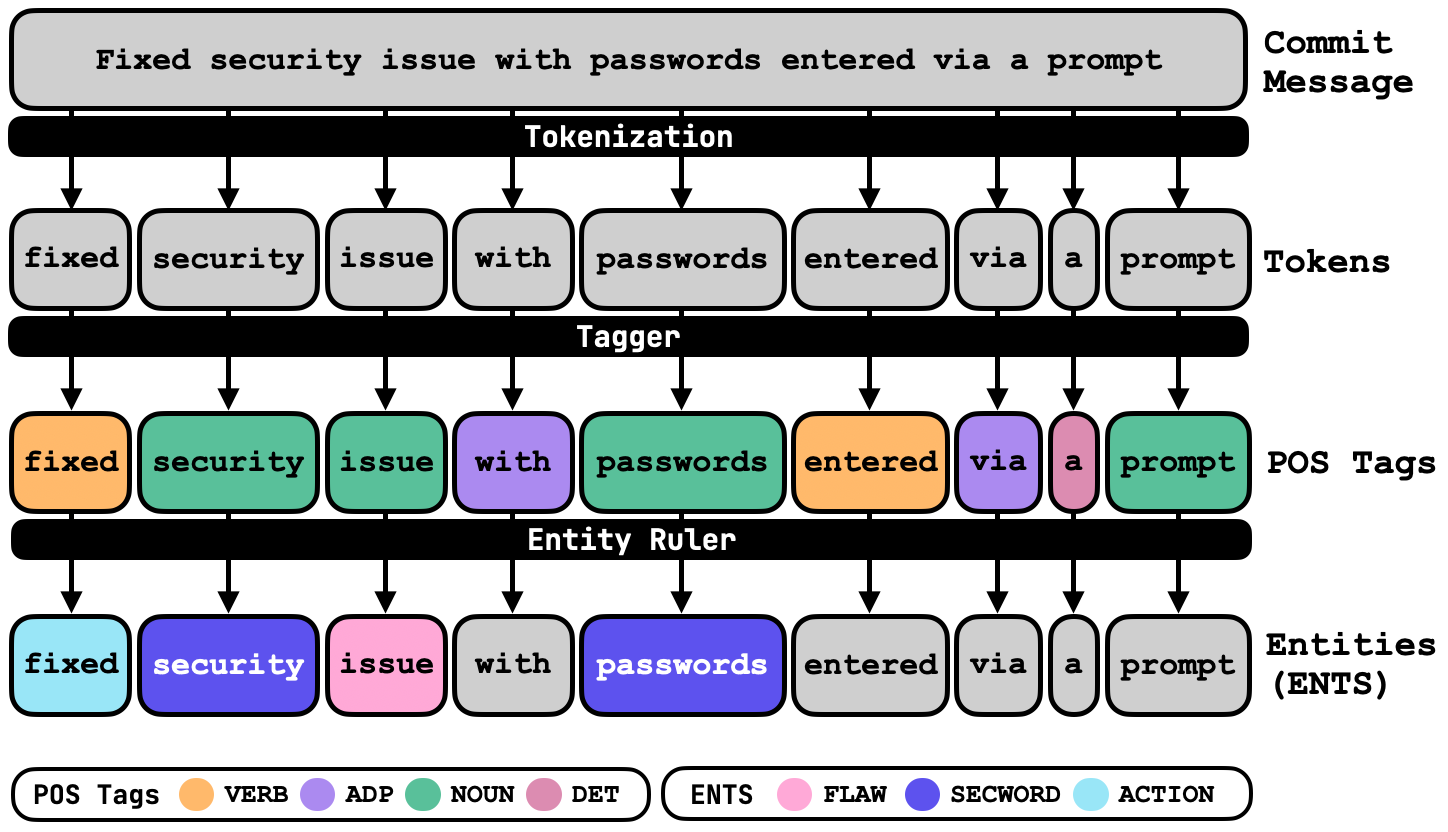
\includegraphics[scale=0.36]{Figures/parsing.png}
    \caption{Extraction Pipeline}\label{fig:parsing}
\end{figure}


\subsubsection{Rules} Fixing security vulnerabilities 
usually involves an ``ACTION'' (one of our category entities, Table~\ref{tab:entities}). Actions can be represented in natural language with verbs such as ``fix'', ``update'', ``patch'', ``mitigate'' and more. Therefore, we created several rules that search for different verbal forms of these words. 
Table~\ref{tab:rules} shows two examples of rules used by our entity ruler. The first rule extracts all the different verbal forms of the word ``fix'' (e.g., ``fix'', ``fixing'', ``fixed'', ``fixes''), i.e., it extracts all variations of the token ``fix'' when its POS tag is a \texttt{VERB}. 

\begin{table}[t!]
\footnotesize
    \centering
        \caption{NER Rule examples. All rules are 
        available in our replication package 
        (\texttt{entity\_ruler/patterns.jsonl}).} 
    \begin{tabular}{ | p{0.25cm} | p{1.25cm} | p{6cm} | }
    \hline
        \textbf{ID} & \textbf{Label} & \textbf{Rule}\\\hline
        R1 & ACTION & \verb|{"label":"ACTION","pattern":[{"LOWER": |\\& & \verb| {"REGEX":"fix.*"},"POS":"VERB"}]}|  \\\hline
        R2 &  VULNID & \verb|{"label":"VULNID","pattern":[{"LOWER":|\\& & \verb|"osv"},{"IS_PUNCT":true,"OP":"?"},|\\& & \verb|{"LOWER":{"REGEX":"\\d{4}"}},|\\& & \verb|{"IS_PUNCT":true,"OP":"?"},|\\& & \verb|{"LIKE_NUM":true}],"id":"OSV"}| 
        \\\hline
    \end{tabular}
    \label{tab:rules}
\end{table}

The second example
illustrates the extraction of different vulnerability IDs. With the 
growth of the open-source security community, different 
ecosystems (e.g., PyPI, NPM, Ruby Gems, and more) are 
starting to report vulnerabilities with their own IDs that 
follow different structures than the usual CVE ID, \verb|CVE-\d-\d{4,7}|. Therefore, we implemented rules to extract the 
different vulnerability IDs (VULNID). One example is R2, 
a rule to extract vulnerability IDs of type (or rule id) OSV for vulnerabilities 
detected with Google's OSS-Fuzzer (e.g., OSV-2023-
27\footnote{https://osv.dev/vulnerability/OSV-2023-27}). 

In  addition, we created a total of $1719$
rules---from words or 
bags of words collected in previous 
work~\cite{10.1145/3133956.3134072,10.1145/3475716.3475781}.  These rules extract security-related words (\texttt{SECWORD}). Many rules were improved after manual 
inspection of commit messages, where (1) we detected erroneous 
extraction when looking at the entities (e.g., due to broken 
tokenization of GitHub Advisory IDs, we had to create several 
different rules based on different tokenization results); or, 
(2) the tool did not extract any entity. This process led us to 
augment the list of category entities and find a set of 
anti-patterns for security commit messages---which is described in detail on Table~\ref{tab:fields}. 


\subsection{Best Practices Analysis (RQ2)}

One way to produce quality 
commit messages is by following best practices or guidelines~\cite{Tian_2022, convcom,linus,atomic}. 
In this part of the study, we explored if some of the available guidelines or standards 
were already under usage and how they could be leveraged to create more structured and complete commit messages for security patches.
We found six main suggestions to produce good commit messages from four sources of guidelines~\cite{convcom,goodcommit,linus,Tian_2022}: (1) conventional commits suggest adding a type as a prefix to the subject/header such as \texttt{fix:} or  \texttt{feat:}~\cite{convcom}; (2) the header should explain the commit in one line and meaningful~\cite{convcom,goodcommit} in the capitalized form, no period in the end and the imperative form~\cite{goodcommit}; (3) the body should explain the problem (what), its impact (why) and the fix (how)~\cite{linus,Tian_2022}; (4) the message should include references to bug-trackers, issues or pull requests (when GitHub is used to manage defects)~\cite{goodcommit}; (5) contacts of the reviewers and reporters~\cite{linus}; and finally, (6) keep commits atomic, i.e., one task per commit~\cite{goodcommit}.

We translated the suggestions mentioned before into seven different compliance checkers, which we used to assess if security engineers are following best practices. Table~\ref{tab:practices} shows the different compliance checkers and their sources. %



\begin{table}[t!]
    \footnotesize
    \centering
        \caption{Best Practices to Write Generic Commit Messages} 

    \begin{tabular}{| p{0.25cm} | p{6cm} | p{1.25cm} | }
    \hline
        \textbf{ID} & \textbf{Best Practice} &  \textbf{Standard}
        \\\hline
        C1 &  The header should be prefixed with a type.  & ~\cite{convcom} \\\hline
        C2 & The message should have a one-line header/subject.  & ~\cite{convcom, linus, goodcommit}\\\hline
        
C3 & The message should have a body.  & ~\cite{linus, goodcommit}\\\hline

C4 & The message should mention the contact of the author (signed-off-by and authored-by).  & ~\cite{linus, goodcommit}\\\hline

C5 & The message should mention the contact of the reviewer (reviewed-by).  & ~\cite{linus, goodcommit}\\\hline

C6 & The message should mention references to issues or pull requests.  & ~\cite{goodcommit}\\\hline

C7 & The message should include references to bug trackers.  & ~\cite{goodcommit}\\\hline

    \end{tabular}
    \label{tab:practices}
\end{table}

\section{SECOM: A Convention for Security Commit Messages and its Validation}~\label{sec:solution}

To address the problems mentioned in the previous section, we propose SECOM, a convention for writing security commit messages; and, validate
its usage with the security 
community. The new convention helps us answer the research question RQ3.  


\subsection{Design of the Convention}

In our empirical study, we observed that although security commit messages do not follow best practices in general, there is a small percentage of people using them---i.e., best practices are being used by some security engineers even if only by a small percentage (Section~\ref{sec:findings}). To facilitate adoption, we created \texttt{SECOM} on top of a well-known group of 
guidelines
for writing good commit messages~\cite{convcom, atomic, linus, goodcommit}.  
Table~\ref{tab:fields} lists and describes the different fields and the reason why each field was considered (\textit{rationale}). For instance, the ``type'' field 
was considered because, according to the Conventional Commits Specification, the header/subject should start with a type ($4.10\%$ of security commit messages include a type at the beginning of the header). In addition, the Google OSV team suggested that type should be indeed considered and proposed a new word for security patches, ``vuln-fix''.

The structure and set of fields 
included in the convention were inferred 
from (1) our empirical analysis  of security
commit messages collected from security patches available in vulnerability
databases such as NVD and OSV; 
(2) feedback collected alongside
the Open Source Security Foundation community; and, (3) previous work on best practices for commit messages~\cite{convcom, atomic, linus, goodcommit,Tian_2022}.

The convention (Listing~\ref{lst:SECOM}) consists of five main 
sections: \textbf{header}, prefixed with the type \texttt{vuln-fix}, 
a simple description of the vulnerability and its identifier 
(when available); \textbf{body}, describes the vulnerability 
(what), its impact (why) and the patch to fix the vulnerability 
(how); \textbf{metadata}, such as type of weakness (CWE-ID), 
severity, CVSS, detection methods, report link, and version 
of the software where the vulnerability was introduced; 
\textbf{contacts}, the names and e-mail contacts of 
the \textbf{reporters} and \textbf{reviewers}; and, finally,
\textbf{references} to bug trackers. The different
sections should be separated with a new line.

\begin{lstlisting}[caption={SECOM Convention},label={lst:SECOM},frame=tlrb]
<type>: <header/subject> (<Vuln-ID>)

<body>
# (what) describe the vulnerability
# (why) describe its impact
# (how) describe the patch/fix

[For Each Weakness in Weaknesses:]
Weakness: <Weakness Name or CWE-ID>
Severity: <Low, Medium, High, Critical>
CVSS: <Severity Numerical Repr. (0-10)>
Detection: <Detection Method>
Report: <Report Link>
Introduced in: <Commit Hash>
[End]

Reported-by: <Name> (<Contact>)
Reviewed-by: <Name> (<Contact>)
Co-authored-by: <Name> (<Contact>)
Signed-off-by: <Name> (<Contact>)

Bug-tracker: <Bug-tracker Link>
OR
Resolves: <Issue/PR No.>
See also: <Issue/PR No.>
\end{lstlisting}

The convention considers security patches should be atomic~\cite{atomic}, i.e., two weaknesses can be patched by the same fix, but if it requires more than one fix, then it should be a different commit. 


\begin{table*}
    \footnotesize
    \centering
    \begin{tabular}{ | p{1.75cm} | p{4cm} | p{11cm} | } 
    \hline
        \textbf{Field} & \textbf{Description} & \textbf{Rationale}\\\hline
        type & Usage of \texttt{vuln-fix} at the beginning of the header/subject to specify the fix is related to a vulnerability. & A \textbf{type} should be assigned to each commit~\cite{convcom}---which will make the identification of vulnerability fixes easier. The \texttt{vuln-fix} value was proposed by the Google OSV team during the feedback collection \textbf{(F)} phase. In addition, 4.10\% of commits follow the
conventional commits convention “<type>(scope):”. \\\hline
        Header/Subject & It should be approximately 50 chars (max 72 chars), capitalized with no period in the end and in the imperative form. & According to the common best practices for commit messages, it is important to summarize the purpose of the commit in one line~\cite{linus, goodcommit}. In our best practices analysis, we observed that $100\%$ of commit messages had a header, but only $38.85\%$ had security-related words and represented an action. \\\hline
        Vuln-ID & When available, e.g., CVE, OSV, GHSA, and other formats. & Adding the vulnerability ID to the header/subject can help to localize the commit responsible for patching the vulnerability faster using features like reflog or shortlog. Only 12.1\% of commit messages included mentions of the vulnerability ID, but 4 out of the 7 participants in \textbf{(F)} phase found including the vulnerability ID in the message important.\\\hline
        Body &  Describe the vulnerability (what), its impact (why), and the patch
    to fix the vulnerability (how) in approximately 75 words (25 words per point). & The body is the most important part of the commit message since it provides space to add details on the problem, impact, and solution~\cite{Tian_2022}. In our empirical analysis, we observed that  59.91\%
    commit messages have a body. However,  only 4031 out of those 6875 cases included security-related words or had meaningful information. \\\hline
        Weakness &  Common Weakness Enumeration ID or name. & The weakness ID provides information on which type of vulnerability can exist in the software. Software patch management teams may proceed differently according to the type of weakness. However, only 0.2\% of messages included this type of information. \\\hline
        Severity &  Severity of the issue (Low, Medium, High, Critical). & Severity can motivate software users to perform patch management faster (in case of critical vulnerabilities)~\cite{Householder2020}. Again, only 1.1\% of commit messages mentioned severity levels. \\\hline
        CVSS &  Numerical (0-10) representation of the severity of a security 
    vulnerability (Common Vulnerability Scoring System). & CVSS allows users to make better sense of the vulnerability severity and can motivate software users to perform patch management faster~\cite{Householder2020}. This field was proposed by a security engineer at OpenSSF that mentioned that sometimes is possible to calculate the score by following the CVSS questionnaire. \\\hline
        Detection &  Detection method (Tool, Manual, etc). & It can be interesting to help future researchers with replication. $4$ out of the $7$ participants in the \textbf{(F)} phase sees value in adding this field (Table~\ref{tab:survey}, RQ2). \\\hline
        Report & Link for vulnerability report, which can back up the lack of information provided in commit messages. & It usually provides more information on the vulnerability exploit or proof-of-concept. We observed that 3 out of the 7 participants would like to see links to reports, \textbf{(F)} phase (RQ1). \\\hline
        Introduced in & Commit hash from the commit that introduced the 
    vulnerability. & Suggested by a survey participant of the (\textbf{F}) phase and used in the OSV Schema~\cite{osv-schema}. In addition, we found SHA keys in 1467 commit messages.\\\hline
        Signed-off by & Name and contact of the person that reported the issue.  & To provide credit to the person that found the problem and ask for more details when necessary. However, only 8.4\% of commit messages were signed off by the respective authors.\\\hline
        Reviewed-by & Name and contact of the person that reviewed and closed the issue. & Reviewers are usually the internal developers or senior developers that review and approve the issues. Only 3.33\% of messages have the reviewers' contact.\\\hline
         Bug-tracker & Link to the issue in an external bug-tracker or \texttt{Resolves... See also:} when GitHub is used to manage issues. & Important to document and discuss the problem, its impact and know which people were involved. In our empirical analysis, we extracted URLs from a total of $929$ commits. \\  
    \hline
    \end{tabular}
    \caption{Fields description and rationale.}
    \label{tab:fields}
\end{table*}

% \textbf{Threats to Validity.} Our sample of participants is small, which may not reflect the entire population. In addition, we only considered participants from the open-source community (i.e., private software developers may not be represented). 

% \textbf{Initial Impact.} SECOM was mentioned as one of 
% the best practices for bulk generation of pull requests 
% to scale vulnerability patching in conferences such as BackHat and Defcon~\cite{blackhat}.


\subsection{Compliance Checklist}

Table~\ref{tab:checklist} provides a checklist (or set of rules) to produce better security commit messages.
For each section of the convention, practitioners will find the fields that should be added to the 
security commit message and questions they should ask when filling them out. We find all the fields important; however, for the sake of prioritization when time is short, we selected some of them as mandatory---which are the ones we think to be most important to detect (type, Vuln-ID), prioritize (Weakness, Severity, CVSS) and understand the message (header, what, why, how). However, practitioners should always try to make security commit messages as detailed as possible. The compliance validation with \texttt{SECOM}'s structure (Listing~\ref{lst:SECOM}) and rules (Table~\ref{tab:checklist}) is currently automated with a tool. In the future, we plan to explore how to generate suggestions to produce better security commit messages or even entire ones to soften the burden of a new standard in maintenance teams.



\begin{table*}
    \footnotesize

    \begin{tabular}{ | p{1.75cm} | p{1.75cm} | p{11.75cm} | p{0.25cm} | } 
    \hline
        \multirow{4}{*}{\textbf{Header}} & type & Did you set the type of the commit as "vuln-fix" at the beginning of the header? & \textbf{M} \\\cline{2-4}
                                & header/subject & Did you summarize the patch changes? & \textbf{M} \\\cline{2-4}
                                & header/subject & Did you summarize the patch changes within $\sim$50 chars?	 & \textbf{O} \\\cline{2-4}
                                & Vuln-ID & Is there a vulnerability ID available? Did you include it between parentheses at the end of the header? & \textbf{M} \\
    \hline\hline
        \multirow{4}{*}{\textbf{Body}} & what & Did you describe the vulnerability or problem in the first sentence of the body?	 & \textbf{M} \\\cline{2-4}
                                & why & Did you describe the impact of the vulnerability in the second sentence of the body?	 & \textbf{M} \\\cline{2-4}
                                & how & Did you describe how the vulnerability was fixed in the third sentence?		 & \textbf{M} \\\cline{2-4}
                                & * & Did you describe the what, why, and how within $\sim$75 words ($\sim$25 words per section)? & \textbf{O} \\
    \hline\hline
        \multirow{6}{*}{\textbf{Metadata}} & Weakness & Can this vulnerability be classified with a type? If so, add it to the metadata section. & \textbf{M} \\\cline{2-4}
                                & Severity & Can infer severity (Low, Medium, High, Critical) for this vulnerability? If so, add it to the metadata section.	 & \textbf{M} \\\cline{2-4}
                                & CVSS & Can you calculate the numerical representation of the severity through the Common Vulnerability Scoring System calculator (https://www.first.org/cvss/calculator/3.0)?			 & \textbf{M} \\\cline{2-4}
                                & Detection & How did you find this vulnerability? (e.g., Tool, Manual, etc) & \textbf{O} \\\cline{2-4}
                                & Report & Is there a link for the vulnerability report available? If so, include it. & \textbf{O} \\\cline{2-4}
                                & Introduced in	 & Include the commit hash from the commit where the vulnerability was introduced. & \textbf{O} \\
    \hline\hline
        \multirow{2}{*}{\textbf{Contacts}} & Reviewed-by & Include the name and/or contact of the person that reviewed and accepted the patch.  & \textbf{O}\\\cline{2-4}
                                    & Signed-off-by	 & Include the name and/or contact of the person that authored the patch.	  & \textbf{M}\\
    \hline\hline
        \multirow{2}{*}{\textbf{Bug-Tracker}} & External & Include the link to the issues or pull requests in the external bug-tracker. & \textbf{O}\\\cline{2-4}
                                    & GitHub	 & Include the links for the issues and pull-requests related to the patch (\texttt{Resolves.. See also:}).	  & \textbf{O}\\
    \hline
    \end{tabular}
    \caption{SECOM Compliance Checklist. [\textbf{M}-Mandatory; \textbf{O}-Optional; \textbf{*}-All fields in the section.]}
    \label{tab:checklist}
\end{table*}

\subsection{SECOM's Application Example}

\texttt{SECOM} is meant to structure and help write more informative and meaningful
security commit messages. In this section, we show an application example of \texttt{SECOM}
to improve the commit message used to document the patch to CVE-2012-0036\footnote{https://nvd.nist.gov/vuln/detail/CVE-2012-0036}, a potential data injection via a crafted URL.

\begin{lstlisting}[caption={Original commit message to fix CVE-2012-0036},label={lst:before},basicstyle=\scriptsize,frame=tlrb]
URL sanitize: reject URLs containing bad data
Protocols (IMAP, POP3 and SMTP) that use the path 
part of a URL in a decoded manner now use the new 
Curl_urldecode() function to reject URLs with 
embedded control codes (anything that is or 
decodes to a byte value less than 32).

URLs containing such codes could easily otherwise 
be used to do harm and allow users to do 
unintended actions with otherwise innocent tools 
and applications. Like for example using a URL 
like pop3://pop3.example.com/1%0d%0aDELE%201 
when the app wants a URL to get a mail and 
instead this would delete one.

This flaw is considered a security 
vulnerability: CVE-2012-0036

Security advisory at: 
http://curl.haxx.se/docs/adv_20120124.html

Reported by: Dan Fandrich
\end{lstlisting}

\begin{lstlisting}[caption={Commit message to fix CVE-2012-0036 (after SECOM's application)},label={lst:after},basicstyle=\scriptsize,frame=tlrb]
vuln-fix: Sanitize URLs to reject malicious data 
(CVE-2012-0036)

Protocols (IMAP, POP3 and SMTP) that use the path 
part of a URL in a decoded manner now use the new 
Curl_urldecode() function to reject URLs with 
embedded control codes (anything that is or 
decodes to a byte value less than 32).
URLs containing such codes could easily otherwise 
be used to do harm and allow users to do 
unintended actions with otherwise innocent tools 
and applications.
Like for example using a URL like 
pop3://pop3.example.com/1%0d%0aDELE%201 when the 
app wants a URL to get a mail and instead this 
would delete one.

Weakness: CWE-89
Severity: High
Detection: Manual
Report: https://curl.se/docs/CVE-2012-0036.html

Reported-by: Dan Fandrich
Signed-off-by: Daniel Stenberg (daniel@haxx.se)

Resolves: #17940
See also: #17937
\end{lstlisting}

Listing~\ref{lst:before} shows the original commit message used to document the code changes
to patch the CVE-2012-0036. Listing~\ref{lst:after} shows an example of the same commit message, 
but if the message had followed the SECOM standard convention and rules. As seen, the header
includes a type, a short message, and the vulnerability ID, followed by the body where a description
of the problem and fix is provided, and later all the information regarding metadata, contacts, and bug trackers are also provided. In the original message, details such as weakness and severity were not provided, which would not allow triage systems to prioritize this patch properly.

\subsection{Standard Validation (RQ3)}

This section describes how we collected feedback (F) from the security community about the proposed convention (SECOM). We prepared a small survey to collect feedback from the open-source security community. 

The survey did not collect any personal data, and we informed that to our participants at the beginning of the form. \texttt{SECOM} was presented and discussed in detail in two working groups of the Open-Source Security Foundation (OpenSSF). 
OpenSSF is an open community where 
security engineers from all over the industry are involved (e.g., Google, Linux Foundation, Intel, RedHat, and more) and on a mission to 
make open-source security better~\cite{OPENSSF-MISSION}. The convention was validated by experienced security engineers involved in the best practices and vulnerability disclosure projects.
At the end
of our discussion, we asked the present security engineers
to provide their feedback on the convention by answering a few questions (see
Table~\ref{tab:survey}). These questions were designed to validate the different fields
we proposed (Q1 and Q2) and to understand the community's opinion on our new solution (Q3-Q5).
For instance, we wanted to understand which field the community finds more important. One 
thing we observed in our manual analysis of commit messages was the mention of the 
process of detection of the vulnerability---sometimes, the tool used to detect the 
vulnerability was mentioned in the message. Since we did not have any strong 
data analysis to backup this decision, we asked the potential users what they 
thought about it.

\begin{table}[!b]
    \footnotesize
    \centering
    \begin{tabular}{ | p{0.25cm} | p{4.5cm} | p{1.75cm} | } 
    \hline
        \textbf{No.} & \textbf{Question} & \textbf{Answer}\\\hline
       Q1 & ``The following pieces of information commonly appear in commit messages of security-related patches.  Which do you find important to include in a security commit message?''  & Vuln-ID, Severity, CVSS, Weakness Type, Report Link\\\hline
        Q2 & ``Security vulnerabilities are usually detected by different means (e.g., manually, static analysis, dynamic analysis, penetration testing, etc.). Do you see value in reporting this information in a security commit message?'' & Yes, No, Unsure\\\hline
        Q3 & ``Would you use this or a similar convention as standard practice in your own work or advocate its use in your team?'' & Yes, No, Unsure\\\hline
        Q4 & ``If you answered "Other" or "Unsure to any of the questions, please explain briefly below.'' & Open \\\hline
        Q5 & ``Please enter any other comments or suggestions below.'' & Open \\
    \hline
    \end{tabular}
    \caption{Survey questions used to validate SECOM.}
    \label{tab:survey}
\end{table}


\section{Findings}~\label{sec:findings}

In this section, we present the main conclusions 
of our empirical analysis of security commit messages 
and the validation of \texttt{SECOM}. 

\subsection*{\textit{RQ1: What information is included in
the commit messages of public security patches?}}


We ran our extraction pipeline (Figure~\ref{fig:parsing}) over a total of $11036$ security commit messages. Table~\ref{tab:entities} shows the number of entities extracted per entity category (\#Entities), the number of commits where entities of each type were found (\#Commits), and the respective percentage of commits (\%Commits). We divided the 
entities into two main sets: security-specific and commit-specific. The tool was able 
to extract key information for both types:
$38.5\%$ of the extracted entities are security-specific, and the remaining $61.5\%$ are commit-specific.

\begin{table}[t!]
\footnotesize
    \centering
        \caption{Extraction Results} 
    \begin{tabular}{| p{2cm} | p{1.25cm} | p{1.5cm} | p{1.5cm} | }
    \hline
        \textbf{Category} & \textbf{\#Entities} & \textbf{\#Commits} & \textbf{\%Commits} \\\hline
SECWORD & 16126 & 6749 & 61.2\%\\\hline
ACTION & 10364 & 6409 & 58.1\%\\\hline
EMAIL & 4738 & 2086 & 18.9\%\\\hline
SHA & 4943 & 1467 & 13.3\%\\\hline
FLAW & 4402 & 2843 & 25.8\%\\\hline
ISSUE & 3561 & 2805 & 25.4\%\\\hline
URL & 1175 & 929 & 8.4\%\\\hline
VULNID & 1799 & 1330 & 12.1\%\\\hline
VERSION & 658 & 571 & 5.2\%\\\hline
DETECTION & 629 & 374 & 3.4\%\\\hline
SEVERITY & 142 & 118 & 1.1\%\\\hline
CWEID & 25 & 23 & 0.2\%\\\hline\hline
\textbf{Total} & 48562 & 10168 & 92.1\%\\\hline
\end{tabular}
    \label{tab:entities}
\end{table}

\textbf{Commit-specific data (COM).} The tool extracted entities for all the $7$ different entity categories classified as commit-specific. A total of $29841$ entities were extracted as commit-specific information. 
A commit usually implies an \emph{action} or \emph{change}. In the case of security, it should imply fixing a vulnerability (corrective maintenance). Yet, only $10364$ entities for verbs (ACTION) were extracted from $6409$ ($58.1\%$) commit messages. Fixing a vulnerability also means fixing a flaw. Our tool extracted mentions of flaws (FLAW) in $2843$ ($25.8\%$) commit messages. 
Mentions of issues (ISSUE) and URLs (URL) can be a good source of external documentation and information, but security engineers rarely mention that information in their commit messages: only $2805$ contained references to issues, and $929$ commit messages contained URLs. 

% Previous work showed that only $38\%$ of security commit messages included security-relevant words~\cite{9678720}. 
\textbf{Security-specific data (SEC).} The tool extracted entities for all the $5$ different entity categories classified as commit-specific. A total of $16126$ security-related words (\texttt{SECWORD}) was collected from $6749$ out of $11036$ ($61.2\%$) commit messages.
Vulnerability IDs (VULNID) were only extracted for $1330$ commit messages, while all patches that integrate our dataset, fix a vulnerability with a known ID. Vulnerability IDs easily map security commits to official reports, which usually provide more details on the vulnerability, product affected, severity, and more. Therefore, they are important to add to commit messages.
It seems that security engineers rarely mention weakness IDs (CWEID)---only $25$ entities were extracted from $23$ commits messages. We suspect that we can often extract the weakness type by looking at the set of entities extracted for the SECWORD category. For instance, in ``fixed xss vulnerability bug by oncellhtmldata'' (commit message from security patch to the GHSA-hf4q-52x6-4p57 vulnerability), we could infer a CWE-79 based on the ``xss'' entity extracted in this message. Severity can be important for security patch management systems to know which security patches to prioritize. If a patch to a critical vulnerability is released, it should be installed as soon as possible. 
However, severity entities (SEVERITY) are rarely included in security commit messages---only extracted from $118$ ($1.1\%$) security commit messages.


\textbf{Finding 1.} Security engineers
use security-related words in
$61.2\%$ of the security commit messages
used to patch software vulnerabilities.



\textbf{Finding 2.} Vulnerability IDs, Weakness IDs and Severity are rarely mentioned 
in security commit messages---although important for manual and automated detection and prioritization. 

Our tool extracted
a total of $48562$ entities from $10168$ out of the $11036$ ($92.1\%$) security commit messages under analysis. For the remaining $868$ of the commit messages, we performed a manual validation of the reason behind of null extraction:
%(Table~\ref{tab:reasons}):

\textbf{Poorly-Written.} We found several types of poorly-written messages reported in previous work~\cite{Tian_2022}. For instance, we found $51$ messages containing only one token (``Single-word''). Some examples are ``update'', ``...'', ``:arrow\_up:'', ``Refactor''. Poorly-written messages usually contain one line without clear information regarding the commit’s purpose (e.g., ``applied updates'', ``backend media''. We found a total of $760$ messages that lacked meaningful information. 

\textbf{Non-Security Related.} Dense message with no clear relationship with security. One example is 
``Support progressive event for dc. This implements the progressive api event fo rthe dc image. This is currently only supported for vardct without extra channels: for
modular and extra channels it's only supported if squeeze is used, and
it may not correctly work with flush yet in that case.''---the commit message of OSV-2021-1606 vulnerability.
We found a total of $97$ commit messages that were hard to relate with security fixes. 

\textbf{Misspelling Issues.} Messages with misspelled english words that would be detected if well written. One example is the message: ``sanitzing user input ''.
However, this kind of issues reflects a very small percentage of the problem.



% \begin{table}[t!]
%     \centering
%         \caption{Reasons why the NER tool failed extraction} 
%     \begin{tabular}{| p{3cm} | p{4cm} | p{0.5cm} | }
%     \hline
%         \textbf{Pattern} & \textbf{Description} &  \textbf{No.}
%         \\\hline
%         Poorly Written  & Containing usually one line without clear information regarding the commit's purpose.   & 760 \\\hline
%         Non-Security Related  & Dense message with no relationship detected with security.  & 97 \\\hline
%         Misspelling Issues & Misspelled english words that lead to unsuccessful extraction. & 11 \\\hline
%         Total &  & 868 \\\hline
%     \end{tabular}
%     \label{tab:reasons}
% \end{table}

\textbf{Finding 3.} No extraction of entities was performed from $8\%$ of security commit messages mainly due to poorly written messages, misspelling issues and no clear connection with security.


\subsection*{\textit{RQ2.  Do security engineers follow best practices to write security commit
messages?}}

We applied $7$ compliance checkers to the commit messages to evaluate if security engineers are using generic best practices to write commit messages since no standard for security exists.

\textbf{C1.} One way of easily marking a commit message for an automated solution is with the usage of a prefix in the header (as the Conventional Commit Convention proposes~\cite{convcom}). In security, this practice was only used in 453 out of 11036 (4.10\%) of commits follow the conventional commits convention ``<type>(scope):'' using prefixes such as ``patch'' or ``fix''.

\textbf{C2.} Headers are important because they are ultimately used to make a quick searches of relevant commits through the git reflog feature. Therefore, it is important that all commit messages have a meaningful and clear header. All the security commit messages (100.00\%) have a one line subject/header. But only 4288 out of 11036 (38.85\%) headers have security-related words (SECWORD) and reflect an action (ACTION).

\textbf{C3.} Previous work has shown that a good commit message needs to clearly mention the problem (what), its impact (why) and how it will be fixed (how)~\cite{Tian_2022}. However, only 6875 out of 11475 (59.91\%) commit messages have a body. Security engineers do not use often security related-words (or vocab) in their body messages since only 4031 out of 11036 (36.53\%) of body messages have SECWORDS.

\textbf{C4.} Crediting the authors of the fixes by signing-off by commits is a very well known practice in security. However, only 925 out of 11036 (8.4\%) commit messages were signed-off by the authors.

\textbf{C5.} Reviewers are usually the internal developers or seniors developers that review and approve the issues. Only 368 out of 11036 (3.33\%) of messages have the reviewers contact.

\textbf{C6.} Issues are good sources of documentation since they sometimes provide details on the discussion of the problem and potential solution. However, only 2805 out of 11036 (25.42\%) commit messages have references to issues.

\textbf{C7.} Same as references to issues, links to bug trackers are also good to mention since they usually provide useful documentation on the problem, fix, severity, and more. But again, only 196 out of 11036 (1.78\%) of commits have references to bug trackers.


\textbf{Finding 4.} Security engineers, do not follow best practices to write security commit messages in general. Even when it seems they are, we concluded that key information is missing---which indicates we need best practices for writing better security commit messages. 


\subsection*{\textit{RQ3. How open is the security community to a new standard for security commit messages?}}

Feedback received from the security community suggests that they see value in SECOM and would like to see it evolve into a standard practice---6 out of the 9 participants responded ``Yes''
to Q3 (``Would you use this or a similar convention
as standard practice in your own work or advocate its use in your team?''), the remaining three participants answered ``Unsure''. None of the participants answered ``No''. 2 out of 9 participants said they did not find valuable to mention how the vulnerability was detected. However, 6 of the 9 participants answered ``yes''. Therefore, we considered the ``Detection'' field in the convention. The vulnerability ID, CWE ID,  and severity are the fields that participants found more important to include 
in the commit message. The least important fields are the CVSS and report link.

\textbf{Finding 5.} The security community sees value in SECOM and aims to adopt it as a standard practice in the future.

The participants that were unsure of SECOM's adoption were mainly concerned with the current practices: ``Folks won't be practicing this style daily, and for drive-by contributions, git messages are likely to be highly ad hoc and idiosyncratic.''. However, we argue that with good automated tools, we can help developers produce better commit messages for security. Writing more structured and informative commit messages is important since, ultimately, it can improve the detection and assessment capabilities of patch triage systems and enable fast patch management. 











\section{Implications and Considerations}\label{sec:discussion}

In this section, we describe the implications of 
our findings, ethical considerations, and how 
SECOM should be used.

\subsection{Dealing With Patch Transparency}\label{sec:transparency}

 Transparency is a double-edged sword. It can be a source of trust for consumers~\cite{Householder2020}, but it also creates vulnerability~\cite{9678720}, and, the need for security is often used to avoid transparency because of the risks that come from it. The reality is that non-transparent processes lead to abuse and make timely patch management a challenge (or even impossible). The CERT Coordinated Vulnerability Disclosure (CVD) guide suggests avoiding silent patches since it hinders public awareness of fixes to software vulnerabilities. This, then, leads to a lack of understanding and trust from developers and to poor triage systems (automated tools are incapable of reasoning about data and detect patches if no key information is provided).
 
 The SECOM convention and best practices purposed in this paper are meant to 
help vendors to produce better documentation and boost the patch 
management phase---responsible for deploying the new changes to the users. We are aware that being too much transparent can make users vulnerable to cyberattacks, but we argue that providing better documentation will help automated tools be more effective and fast for software security patch management. So, OSS users and companies can benefit from an automated solution by being aware 
of the fixes as soon as they are developed, which is usually one week earlier than
the disclosure~\cite{10.1145/3133956.3134072}.  

Experienced security engineers should determine when and not when to provide details. If development systems are private, 
then no major risks are attached to providing a detailed security commit message (in principle, we do not account for internal attackers). However, when a critical vulnerability is to be patched in open-source software of wide use, then security engineers should carefully decide which details to include in the commit message. They should provide enough information to users understand its criticality but not enough to attackers leverage.

One thing we do not advocate is the documentation of exploits since this would clearly benefit malicious attackers. That kind of information should be released later, after providing time for the users to deploy the patch.

\subsection{The Burden of a New Standard}

Applying new best practices is usually taken as a burden by the software and security communities, but it is also how we prevent and solve current challenges. As we mentioned before, well-structured and complete documentation is crucial to create trust between different parties and faster patch management---to decrease the user's exposure window. Therefore, we, as a team, and part of the software engineering community, are working on automated solutions for compliance validation and the generation of commit messages to reduce the bottleneck that our standard could introduce. \texttt{SECOM} can also be leveraged to guide other solutions to generate commit messages~\cite{7203049}. It is also important to notice that the open-source security community sees value in SECOM and aims to adopt it as a standard practice in the future. In fact, some security researchers are already using it and considering it as standard best practice~\cite{blackhat}, and more than 2k commit messages were produced following our solution.

\subsection{Need for Better Patch Documentation}

Previous work has shown that the software patch detection problem could not be solved only with security commit messages (or other types of metadata)~\cite{DBLP:journals/corr/abs-1806-05893,9678720}---which we agree. The solution proposed is to focus on code information instead. One study proposed a mixed solution~\cite{SSPatcher2022}. However, we think that focusing on code information will not fix the issue soon due to the complexity of the patterns under analysis (software vulnerability), the approaches gaps (e.g., machine learning, deep learning~\cite{9448435}), the diversity of weaknesses and many more. Instead, we can make an extra effort to provide better documentation and not only improve automated solutions but also build trust between vendors and users---which we argue will ultimately build a safer environment.


\section{Threats to Validity}\label{sec:t2v}

This section discusses the study's potential threats to validity.

\textbf{Internal Validity:}  In the survey study, our sample of participants is small, which may not reflect the entire population. However, we ensured that all the answers come from a reliable and expert source (OpenSSF). In addition, we only considered participants from the open-source community (i.e., private software developers may not be represented).

\textbf{External Validity:} We did not check for all the rules described in the standards considered. Therefore, our conclusion may not reflect the entire ground truth. But, we did check the most important rules, the ones related to having a type, header, and body in the commit message which improves the commit messages considerably.


% This section looks pretty short. Normally needs to be divided into External Validity (generalizability, related to the diversity of the data) and Internal Validity (possible flaws in the design, methodology, data collection, measurement, representation of constructs used). The one threat that was mentioned is internal validity, related to reliability. Is this section complete, or to be completed. At least one could say "the biggest internal threat to the study is ... (the one you mentioned)", and then comment on external validity, whether the conclusions can be generalized to all security commit messages, or a subset (e.g, open-source), or even a smaller subset of OS typified by the data collected.


\section{Related Work}\label{sec:rw}

This section summarizes previous research work in the fields
of Software Security Patch Management, Software Security Patch
Detection and Commit Message Analysis.

\subsection{Software Security Patch Management}

Software security patch management is the process of identifying, acquiring,
testing, installing, and verifying security patches for software products and systems~\cite{DISSANAYAKE2022106771}. 
Security patches are considered the most effective strategy to mitigate software vulnerabilities~\cite{DISSANAYAKE2022106771,SOFT-PATCH-MANAG-NIST,10.1145/2660267.2660329}.
They are prioritized over non-security patches as they aim to protect users from cyberattacks~\cite{SOFT-PATCH-MANAG-NIST}. 
Yet, one important challenge still prevails, the \emph{lack of efficient patch triage systems} to identify and prioritize security patches~\cite{Zhang2021AnIO, SSPatcher2022,hacker-news-patches,DBLP:conf/soups/LiRMMC19}: current processes are largely manual (time-consuming) and prone to ignore important bug fixes such as the one behind Equifax~\cite{failed-to-deploy-patch}.
Figure~\ref{fig:cycle} shows part of the patch management process: \emph{1)} vendors release a patch to mitigate a vulnerability previously identified or reported; \emph{2)} automated or manual systems identify and prioritize the patch and trigger patch deployment; \emph{3)} the patch is deployed successfully into the users' machines. In this paper, we propose a solution that can improve the understanding and identification of security patches for automated and manual triage systems, which can consequently decrease the time users are exposed to vulnerabilities. 
Silent fixes, i.e., software vulnerabilities patched without any release note, hinder security patch management since they leave users unaware of the new patches and their criticality~\cite{Householder2020}---knowledge about the fix is key for successful patch deployment. 
Previous work has shown that $56.7\%$ of the security commit messages are documented poorly~\cite{10.1145/3593434.3593481}, which hinders the different triage systems tasks.
This paper presents a solution to make security commit messages more informative and enable the effectiveness of patch management processes.

\subsection{Software Security Patch Detection}

Version control systems are used to maintain a record of code changes
and manage access to codebase development artifacts~\cite{10.1145/2950290.2950364}. As with any type of code changes, security patches are pushed to codebases through commits. Each commit contains changes to source code and a message explaining what changes
are made and why~\cite{883028,Tian_2022}. Over the past years, many approaches have emerged to detect security patches through metadata (e.g., commit logs, commit metadata, and associated reports) and code changes. Here, we only
mention approaches considering commit logs (or messages).
\emph{Reis et al.} detected security patches for 16 types of weaknesses in commit messages by applying different regular expressions per each kind of weakness~\cite{reis2017secbench}.
% Researchers from the security industry 
% % (Zhou and Sharma 2017; Sabetta and Bezzi
% % 2018) (from SourceClear, Inc., and SAP, respectively)
% have presented early investigations on the prediction of security issues in relation with
% commit changes.
\emph{Zhou and Asankhaya}  leveraged regular expressions to identify
features for predicting security-relevant commits in commit logs,
commit metadata, and associated bug reports. Features are vectorized and learned by word2vec~\cite{10.1145/3106237.3117771}. 
\emph{Sabetta and Bezzi} extended previous work by considering code changes as well~\cite{DBLP:journals/corr/abs-1807-02458}---which led to considerable performance improvements.
\emph{Sawadogo et al.} proposed SSPCatcher, a co-Training-based approach to catch
security patches as part of an automatic monitoring service of code repositories~\cite{SSPatcher2022}. Detection is based on the result of two Support Vector Machine classifiers: 1) one trained with commit logs; and, 2) one trained with code features. In order to identify a new security patch, both 
classifiers have to be in agreement. In this study, we do not propose a new model or approach to detect security patches. Instead, we empirically analyze security commit messages and propose a standard that can improve the effectiveness of the different triage systems tasks (e.g., detection, assessment, and prioritization).

\subsection{Security Commit Message Analysis and Standards}

Previous work has shown that only $38\%$ of security commit messages used to ``silently'' patch software vulnerabilities in the past included security-related words~\cite{9678720}. In this work, 
we analyzed the commit messages attached to all security patches to known software vulnerabilities instead of only focusing on silent fixes. As mentioned before, we were unable 
to find a convention or standard for security commit messages. Instead, we only 
found guidelines and specifications for general commit messages. The preliminary results
of this study were published before~\cite{9796324}. This paper is an extension and 
detailed report on how we analyzed the data, the results, and the design of our solution.

\section{Conclusions and Future Work}\label{sec:fw}

In this study, we observed that security commit messages integrate some relevant information for automated and manual triage systems but not enough to map them to bug reports or know which patches to prioritize. We also observed that no standards exist for security and that security engineers usually do not follow best practices. This paper presents a solution for 
the lack of structure, and key information in the  
commit messages of security fixes. we built SECOM, a convention for security commit messages, based on our empirical analysis findings and the open-source security community feedback and approval. 

Although part of the security community worries about the attacks that potentially will come from transparency, there seems to be space in the security community for a new standard that is already helping security engineers produce better security commit messages. However, it should be used carefully and consider the software vulnerability impact and time response of the maintenance team. 
%
In the future, we plan to release automated solutions for compliance validation and message generation to reduce the burden that a new best practice can introduce in the patching and disclosure life-cycle. 
